\section{Análisis del sistema}

\subsection{Reuniones con el cliente y detalles por afinar}


\begin{figure}[htb]
\begin{center}
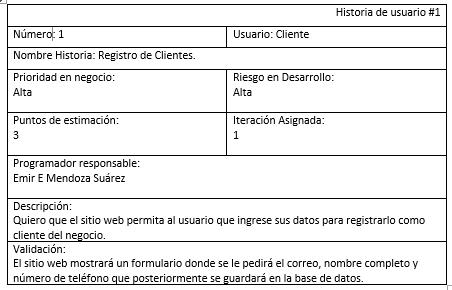
\includegraphics[width=11cm]{./imagenes/tablas/HU1.png}
\end{center}

\end{figure}


\begin{figure}[htb]
\begin{center}
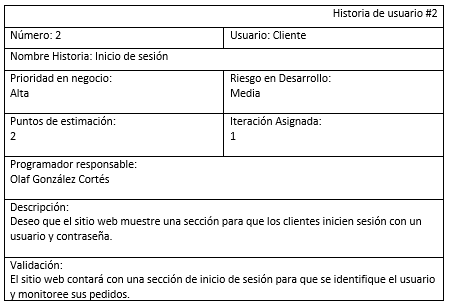
\includegraphics[width=11cm]{./imagenes/tablas/HU2.png}
\end{center}

\end{figure}

\newpage


\begin{figure}[htb]
\begin{center}
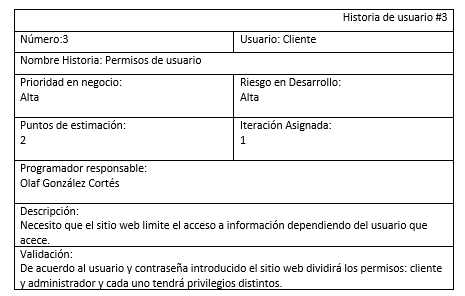
\includegraphics[width=11cm]{./imagenes/tablas/HU3.png}
\end{center}

\end{figure}


\begin{figure}[htb]
\begin{center}
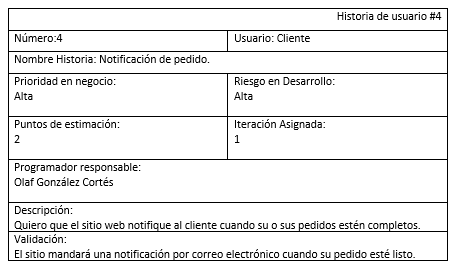
\includegraphics[width=11cm]{./imagenes/tablas/HU4.png}
\end{center}

\end{figure}

\newpage

\begin{figure}[htb]
\begin{center}
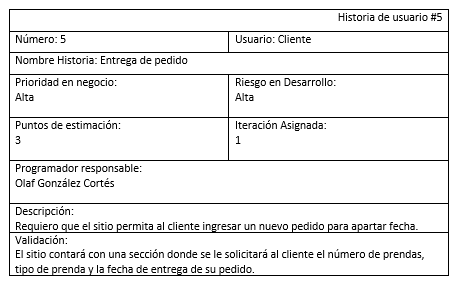
\includegraphics[width=11cm]{./imagenes/tablas/HU5.png}
\end{center}

\end{figure}



\begin{figure}[htb]
\begin{center}
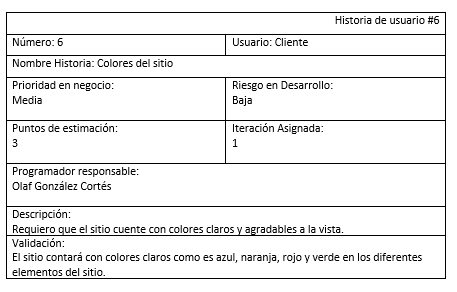
\includegraphics[width=11cm]{./imagenes/tablas/HU6.png}
\end{center}

\end{figure}

\newpage

\begin{figure}[htb]
\begin{center}
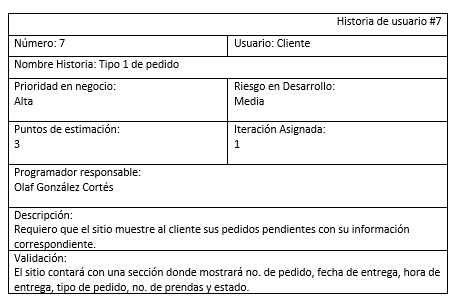
\includegraphics[width=11cm]{./imagenes/tablas/HU7.png}
\end{center}

\end{figure}



\begin{figure}[htb]
\begin{center}
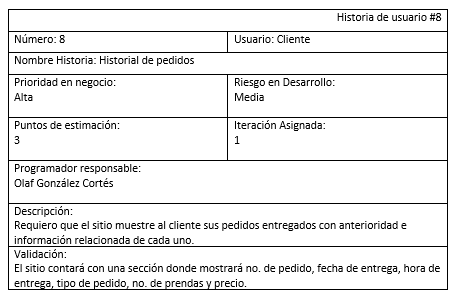
\includegraphics[width=11cm]{./imagenes/tablas/HU8.png}
\end{center}

\end{figure}
\newpage


\begin{figure}[htb]
\begin{center}
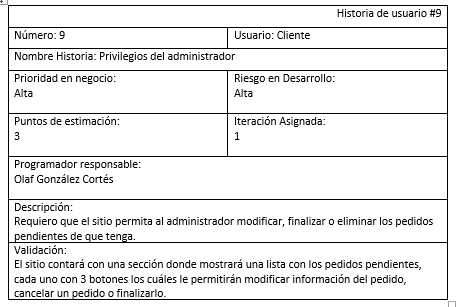
\includegraphics[width=11cm]{./imagenes/tablas/HU9.png}
\end{center}

\end{figure}



\begin{figure}[htb]
\begin{center}
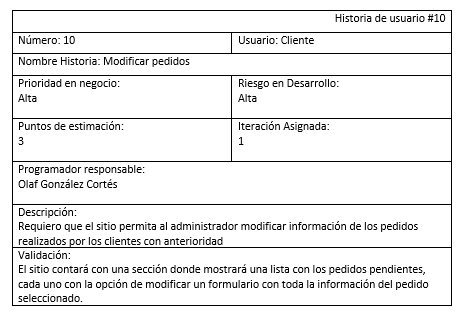
\includegraphics[width=11cm]{./imagenes/tablas/HU10.png}
\end{center}

\end{figure}

\newpage

\subsection{Requisitos funcionales y no funcionales IEEE 830}

\begin{figure}[htb]
\begin{center}
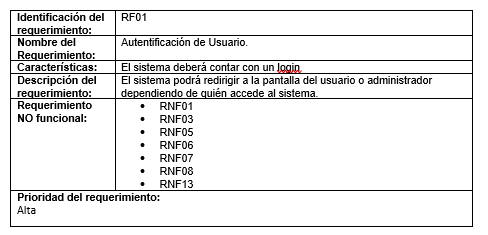
\includegraphics[width=11cm]{./imagenes/tablas/RF01.png}
\end{center}

\end{figure}



\begin{figure}[htb]
\begin{center}
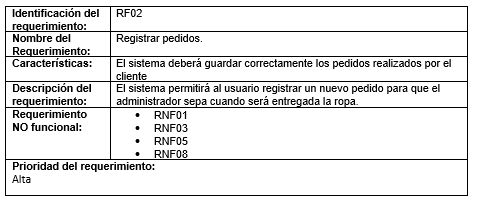
\includegraphics[width=11cm]{./imagenes/tablas/RF02.png}
\end{center}

\end{figure}




\begin{figure}[htb]
\begin{center}
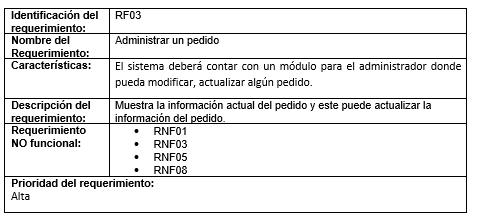
\includegraphics[width=11cm]{./imagenes/tablas/RF03.png}
\end{center}

\end{figure}

\newpage



\begin{figure}[htb]
\begin{center}
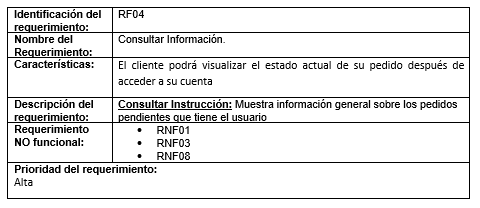
\includegraphics[width=11cm]{./imagenes/tablas/RF04.png}
\end{center}

\end{figure}



\begin{figure}[htb]
\begin{center}
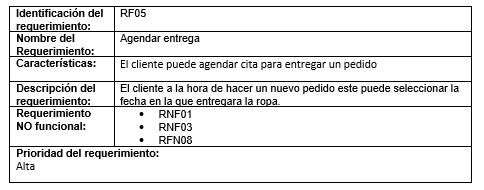
\includegraphics[width=11cm]{./imagenes/tablas/RF05.png}
\end{center}

\end{figure}




\begin{figure}[htb]
\begin{center}
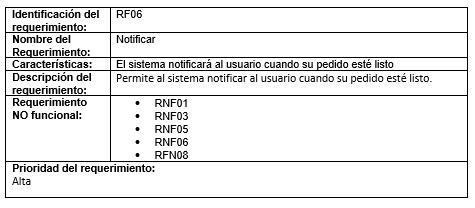
\includegraphics[width=11cm]{./imagenes/tablas/RF06.png}
\end{center}

\end{figure}

\newpage


\begin{figure}[htb]
\begin{center}
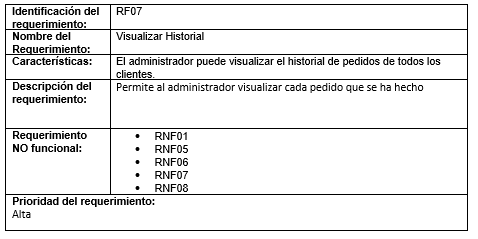
\includegraphics[width=11cm]{./imagenes/tablas/RF07.png}
\end{center}

\end{figure}



\begin{figure}[htb]
\begin{center}
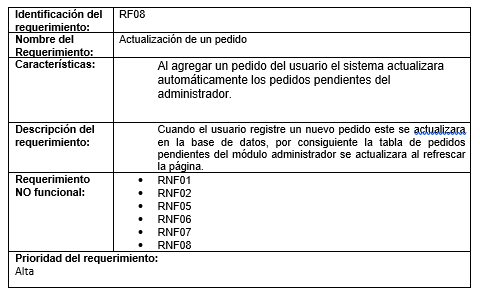
\includegraphics[width=11cm]{./imagenes/tablas/RF08.png}
\end{center}

\end{figure}

\newpage



\begin{figure}[htb]
\begin{center}
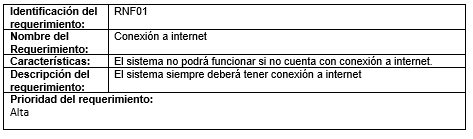
\includegraphics[width=11cm]{./imagenes/tablas/RNF01.png}
\end{center}

\end{figure}




\begin{figure}[htb]
\begin{center}
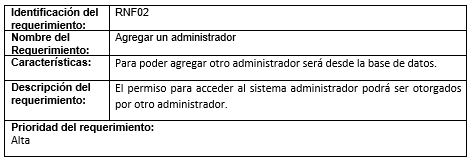
\includegraphics[width=11cm]{./imagenes/tablas/RNF02.png}
\end{center}

\end{figure}





\begin{figure}[htb]
\begin{center}
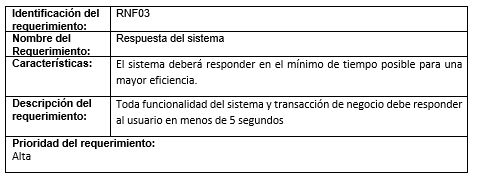
\includegraphics[width=11cm]{./imagenes/tablas/RNF03.png}
\end{center}

\end{figure}


\newpage


\begin{figure}[htb]
\begin{center}
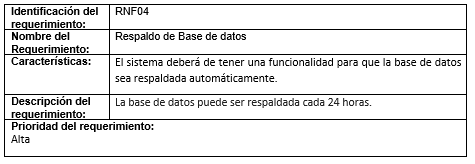
\includegraphics[width=11cm]{./imagenes/tablas/RNF04.png}
\end{center}

\end{figure}






\begin{figure}[htb]
\begin{center}
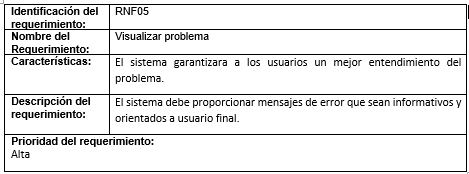
\includegraphics[width=11cm]{./imagenes/tablas/RNF05.png}
\end{center}

\end{figure}





\begin{figure}[htb]
\begin{center}
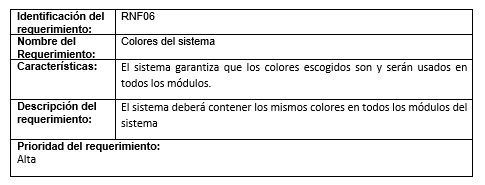
\includegraphics[width=11cm]{./imagenes/tablas/RNF06.png}
\end{center}

\end{figure}

\newpage



\begin{figure}[htb]
\begin{center}
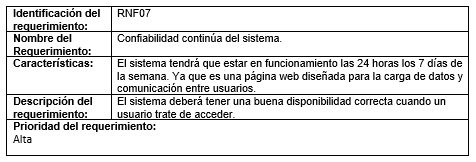
\includegraphics[width=11cm]{./imagenes/tablas/RNF07.png}
\end{center}

\end{figure}





\begin{figure}[htb]
\begin{center}
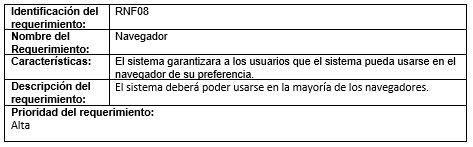
\includegraphics[width=11cm]{./imagenes/tablas/RNF08.png}
\end{center}

\end{figure}





\begin{figure}[htb]
\begin{center}
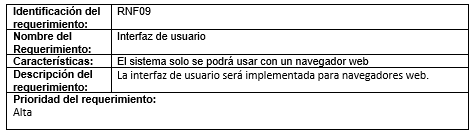
\includegraphics[width=11cm]{./imagenes/tablas/RNF09.png}
\end{center}

\end{figure}



\newpage


\begin{figure}[htb]
\begin{center}
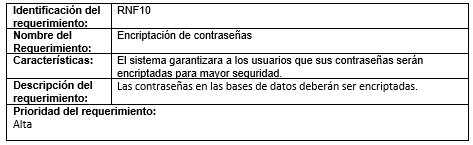
\includegraphics[width=11cm]{./imagenes/tablas/RNF10.png}
\end{center}

\end{figure}





\begin{figure}[htb]
\begin{center}
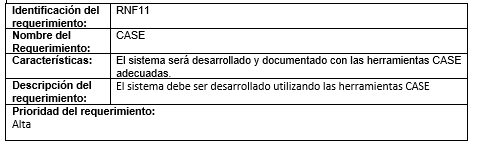
\includegraphics[width=11cm]{./imagenes/tablas/RNF11.png}
\end{center}

\end{figure}





\begin{figure}[htb]
\begin{center}
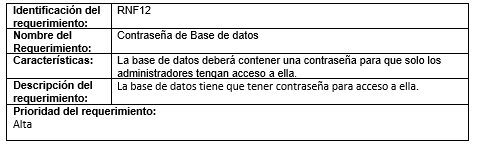
\includegraphics[width=11cm]{./imagenes/tablas/RNF12.png}
\end{center}

\end{figure}


\newpage


\begin{figure}[htb]
\begin{center}
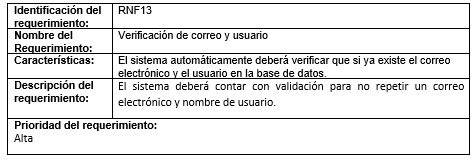
\includegraphics[width=11cm]{./imagenes/tablas/RNF13.png}
\end{center}

\end{figure}





\begin{figure}[htb]
\begin{center}
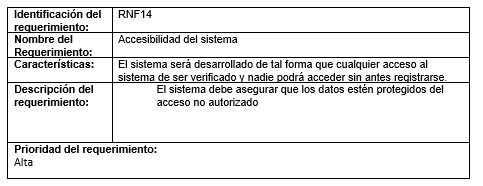
\includegraphics[width=11cm]{./imagenes/tablas/RNF14.png}
\end{center}

\end{figure}


\subsection{Métodos formales (importancia y uso)}
Son un tipo particular de la técnica basada en las matemáticas para la especificación formal, desarrollo y verificación formal de los sistemas de software y hardware. El uso de métodos formales para el diseño de software y hardware está motivado por la expectativa de que, la realización de un análisis matemático adecuado puede contribuir a la fiabilidad y robustez de un diseño. 

\subsubsection{Requisitos en lógica de predicados}

